%==============================================================================
% Chapitre 45 - Le sertissage
%==============================================================================

\section{Introduction}

Le projectile est généralement maintenu dans le collet de l'étui par la seule
tension exercée par celui-ci.

Dans certaines situations, ce maintien peut être renforcé par une opération
appelée sertissage.

Le sertissage constitue une étape importante dans la fabrication de nombreuses
munitions.

\begin{aretenir}

Le sertissage consiste à déformer légèrement le collet afin d'améliorer le
maintien du projectile.

\end{aretenir}

\section{Objectifs du sertissage}

Le sertissage peut remplir plusieurs fonctions :

\begin{itemize}
    \item empêcher le déplacement du projectile ;
    \item améliorer la résistance aux chocs ;
    \item résister aux effets du recul ;
    \item améliorer la régularité du départ du projectile ;
    \item faciliter le fonctionnement de certaines armes.
\end{itemize}

Selon les applications, l'importance de ces fonctions varie.

\section{Pourquoi maintenir le projectile ?}

Avant le tir, le projectile est soumis à diverses contraintes :

\begin{itemize}
    \item manipulations ;
    \item vibrations ;
    \item chocs ;
    \item accélérations ;
    \item recul.
\end{itemize}

Un maintien insuffisant peut provoquer des déplacements indésirables.

\section{Déplacement vers l'intérieur}

Dans certains cas, le projectile peut s'enfoncer davantage dans l'étui.

Ce phénomène réduit le volume disponible pour la poudre.

Il peut alors entraîner :

\begin{itemize}
    \item une augmentation de la pression ;
    \item une modification des performances ;
    \item des risques de surpression.
\end{itemize}

\section{Déplacement vers l'extérieur}

Le projectile peut également sortir partiellement de l'étui.

Ce phénomène est particulièrement redouté dans certains revolvers puissants.

Une cartouche trop longue peut alors :

\begin{itemize}
    \item gêner la rotation du barillet ;
    \item provoquer un incident de fonctionnement.
\end{itemize}

\section{Principe du sertissage}

Le sertissage consiste à déformer légèrement le collet autour du projectile.

Cette déformation augmente l'effort nécessaire pour déplacer celui-ci.

Le maintien devient alors plus important.

\section{Sertissage et tension de collet}

Le sertissage ne remplace pas une bonne tension de collet.

Dans la plupart des cas :

\begin{itemize}
    \item la tension de collet assure l'essentiel du maintien ;
    \item le sertissage constitue un complément.
\end{itemize}

\begin{aretenir}

Un sertissage ne doit pas compenser un collet mal dimensionné.

\end{aretenir}

\begin{figure}[htbp]
\centering

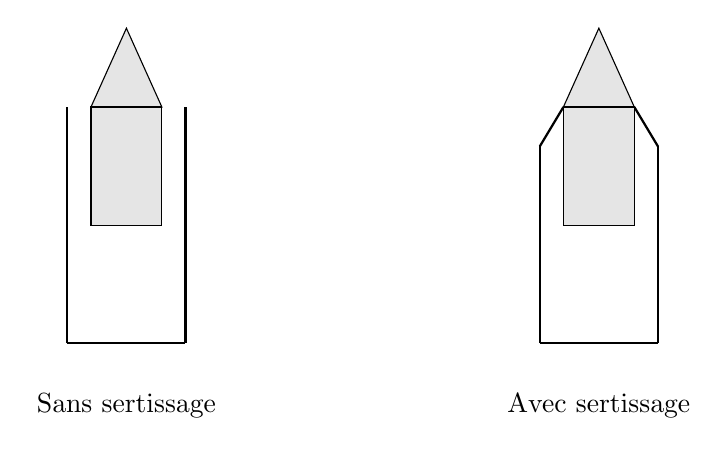
\begin{tikzpicture}[scale=1]

% Sans sertissage
\begin{scope}

\draw[thick] (0,0) -- (0,3);
\draw[thick] (1.5,0) -- (1.5,3);

\draw[thick] (0,0) -- (1.5,0);

% Projectile
\draw[fill=gray!20]
(0.3,3) --
(0.75,4) --
(1.2,3) --
cycle;

\draw[fill=gray!20]
(0.3,1.5) rectangle (1.2,3);

\node at (0.75,-0.8) {Sans sertissage};

\end{scope}

% Avec sertissage
\begin{scope}[xshift=6cm]

\draw[thick] (0,0) -- (0,2.5);
\draw[thick] (1.5,0) -- (1.5,2.5);

\draw[thick] (0,0) -- (1.5,0);

% Collet replié
\draw[thick] (0,2.5) -- (0.3,3);
\draw[thick] (1.5,2.5) -- (1.2,3);

% Projectile
\draw[fill=gray!20]
(0.3,3) --
(0.75,4) --
(1.2,3) --
cycle;

\draw[fill=gray!20]
(0.3,1.5) rectangle (1.2,3);

\node at (0.75,-0.8) {Avec sertissage};

\end{scope}

\end{tikzpicture}

\caption{Influence du sertissage sur le maintien du projectile dans le collet.}
\label{fig:sertissage_principe}

\end{figure}

\section{Le sertissage roulé}

Le sertissage roulé (\emph{roll crimp}) consiste à rabattre légèrement le bord
du collet vers l'intérieur.

Cette technique est fréquemment utilisée pour :

\begin{itemize}
    \item les munitions de revolver ;
    \item certaines cartouches de chasse ;
    \item certaines cartouches à fort recul.
\end{itemize}

\section{Le sertissage conique}

Le sertissage conique (\emph{taper crimp}) réduit progressivement le diamètre
du collet.

Cette méthode est couramment utilisée pour :

\begin{itemize}
    \item les cartouches d'armes de poing modernes ;
    \item les cartouches prenant leur feuillure sur le collet.
\end{itemize}

\begin{figure}[htbp]
\centering

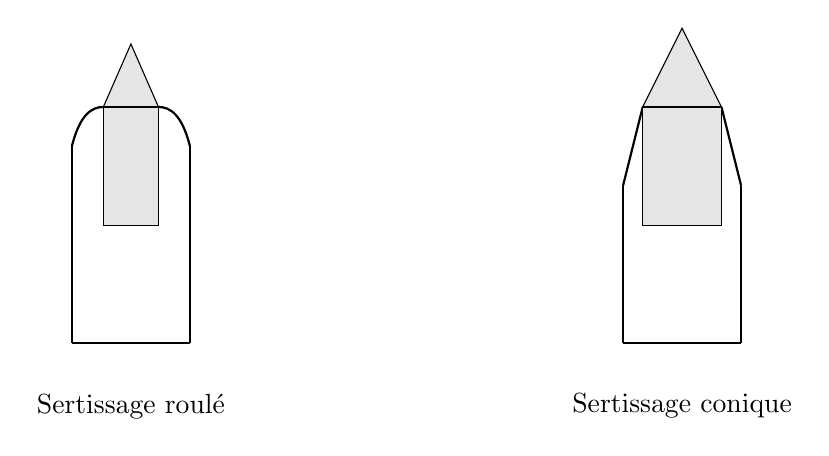
\begin{tikzpicture}[scale=1]

% Roll Crimp
\begin{scope}

\draw[thick] (0,0) -- (0,2.5);
\draw[thick] (1.5,0) -- (1.5,2.5);

\draw[thick] (0,0) -- (1.5,0);

% Repli du collet
\draw[thick]
(0,2.5)
.. controls (0.1,2.9) and (0.25,3.0) ..
(0.4,3.0);

\draw[thick]
(1.5,2.5)
.. controls (1.4,2.9) and (1.25,3.0) ..
(1.1,3.0);

% Projectile
\draw[fill=gray!20]
(0.4,3) --
(0.75,3.8) --
(1.1,3) --
cycle;

\draw[fill=gray!20]
(0.4,1.5) rectangle (1.1,3);

\node at (0.75,-0.8) {Sertissage roulé};

\end{scope}

% Taper Crimp
\begin{scope}[xshift=7cm]

\draw[thick] (0,0) -- (0,2.0);
\draw[thick] (1.5,0) -- (1.5,2.0);

\draw[thick] (0,0) -- (1.5,0);

% Réduction progressive
\draw[thick] (0,2.0) -- (0.25,3.0);
\draw[thick] (1.5,2.0) -- (1.25,3.0);

% Projectile
\draw[fill=gray!20]
(0.25,3) --
(0.75,4) --
(1.25,3) --
cycle;

\draw[fill=gray!20]
(0.25,1.5) rectangle (1.25,3);

\node at (0.75,-0.8) {Sertissage conique};

\end{scope}

\end{tikzpicture}

\caption{Comparaison entre un sertissage roulé et un sertissage conique.}
\label{fig:roll_taper_crimp}

\end{figure}

\section{Le sertissage d'usine}

Certaines munitions reçoivent un sertissage réalisé lors de leur fabrication.

Les procédés employés permettent une excellente répétabilité.

Ils contribuent à la régularité des performances.

\section{Gorge de sertissage}

Certains projectiles possèdent une gorge spécifique appelée :

\begin{quote}
gorge de sertissage
\end{quote}

ou :

\begin{quote}
cannelure
\end{quote}

Cette zone facilite l'application du sertissage.

\begin{figure}[htbp]
\centering

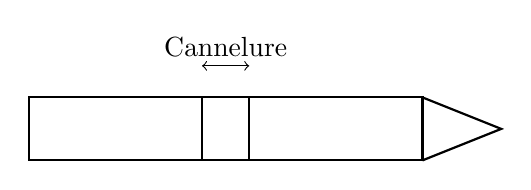
\begin{tikzpicture}[scale=1]

% Projectile
\draw[thick]
(0,0) rectangle (5,0.8);

\draw[thick]
(5,0)
-- (6,0.4)
-- (5,0.8);

% Cannelure
\draw[thick] (2.2,0) -- (2.2,0.8);
\draw[thick] (2.8,0) -- (2.8,0.8);

\draw[<->] (2.2,1.2) -- (2.8,1.2);

\node[above] at (2.5,1.2) {Cannelure};

\end{tikzpicture}

\caption{Exemple de cannelure destinée au sertissage.}
\label{fig:cannelure}

\end{figure}

\section{Influence sur la pression}

Le sertissage augmente généralement la résistance initiale au mouvement du
projectile.

Cette résistance peut modifier :

\begin{itemize}
    \item la montée en pression ;
    \item la combustion de la poudre ;
    \item la vitesse initiale.
\end{itemize}

\section{Influence sur la précision}

L'effet du sertissage sur la précision dépend fortement du contexte.

Selon les armes et les chargements :

\begin{itemize}
    \item il peut améliorer la régularité ;
    \item il peut être sans effet notable ;
    \item il peut parfois dégrader les résultats.
\end{itemize}

L'expérimentation reste souvent nécessaire.

\section{Applications typiques}

Le sertissage est fréquemment utilisé pour :

\begin{itemize}
    \item les revolvers ;
    \item les armes à levier ;
    \item certaines armes semi-automatiques ;
    \item certaines munitions militaires.
\end{itemize}

\section{Le cas du rechargement}

En rechargement, le sertissage doit être appliqué avec discernement.

Un sertissage excessif peut :

\begin{itemize}
    \item déformer le projectile ;
    \item détériorer l'étui ;
    \item nuire à la précision.
\end{itemize}

\section{Quand sertir ?}

Il n'existe pas de règle universelle.

Le besoin dépend notamment :

\begin{itemize}
    \item du type d'arme ;
    \item du projectile ;
    \item du recul ;
    \item du mode d'alimentation ;
    \item de l'usage recherché.
\end{itemize}

\section{Vers les calibres}

Le sertissage constitue l'une des nombreuses caractéristiques pouvant varier
d'une cartouche à l'autre.

Pour comprendre la diversité des munitions existantes, il est maintenant
nécessaire d'aborder la notion de calibre.

\section{À retenir}

\begin{aretenir}

\begin{itemize}
    \item Le sertissage améliore le maintien du projectile.
    \item Il complète la tension de collet.
    \item Le sertissage roulé et le sertissage conique sont les plus répandus.
    \item Un sertissage excessif peut être nuisible.
    \item Son influence dépend fortement de l'application considérée.
\end{itemize}

\end{aretenir}
